\chapter{Debugger DDD}

\begin{chapquote}{Autor desconhecido}
``Meu software nunca possui bugs. Ele só
desenvolve recursos aleatórios.''
\end{chapquote}

Um depurador permite ao usuário controlar a execução de um programa, examinar variáveis, outra memória (ou seja, espaço na pilha) e exibir a saída do programa (se houver). O GNU Data Display Debugger de código aberto (DDD\footnote{Para mais informações, consulte: https://pt.wikipedia.org/wiki/Data\_Display\_Debugger}) é um front-end visual para o GNU Debugger (GDB\footnote{Para mais informações, consulte: https://pt.wikipedia.org/wiki/GNU\_Debugger}) e está amplamente disponível. Outros depuradores podem ser facilmente usados, se desejado.

Somente os comandos básicos do depurador são abordados neste capítulo. O depurador DDD possui muitos outros recursos e opções não abordados aqui. À medida que você ganha experiência, vale a pena revisar a documentação do DDD, mencionada no Capítulo \ref{cap1}, para aprender mais sobre os recursos adicionais, a fim de ajudar a melhorar a eficiência geral da depuração.

A funcionalidade do DDD pode ser estendida usando vários plug-ins. Os plug-ins não são necessários e não serão abordados neste capítulo.

Este capítulo aborda o uso do depurador GNU DDD como uma ferramenta. O processo lógico de como depurar um programa não é abordado neste capítulo.

\section{Iniciando o DDD}
O depurador \textbf{ddd} é iniciado com o arquivo executável. O programa deve ser montado e vinculado às opções corretas (conforme observado no capítulo anterior). Por exemplo, usando o programa exemplo anterior, por exemplo, o comando seria:
\begin{verbatim}
ddd primeiro
\end{verbatim}

Ao iniciar o DDD/GDB, algo semelhante à tela, mostrada abaixo, deve ser exibida (com o código-fonte apropriado exibido).

\begin{figure}
\begin{center}
		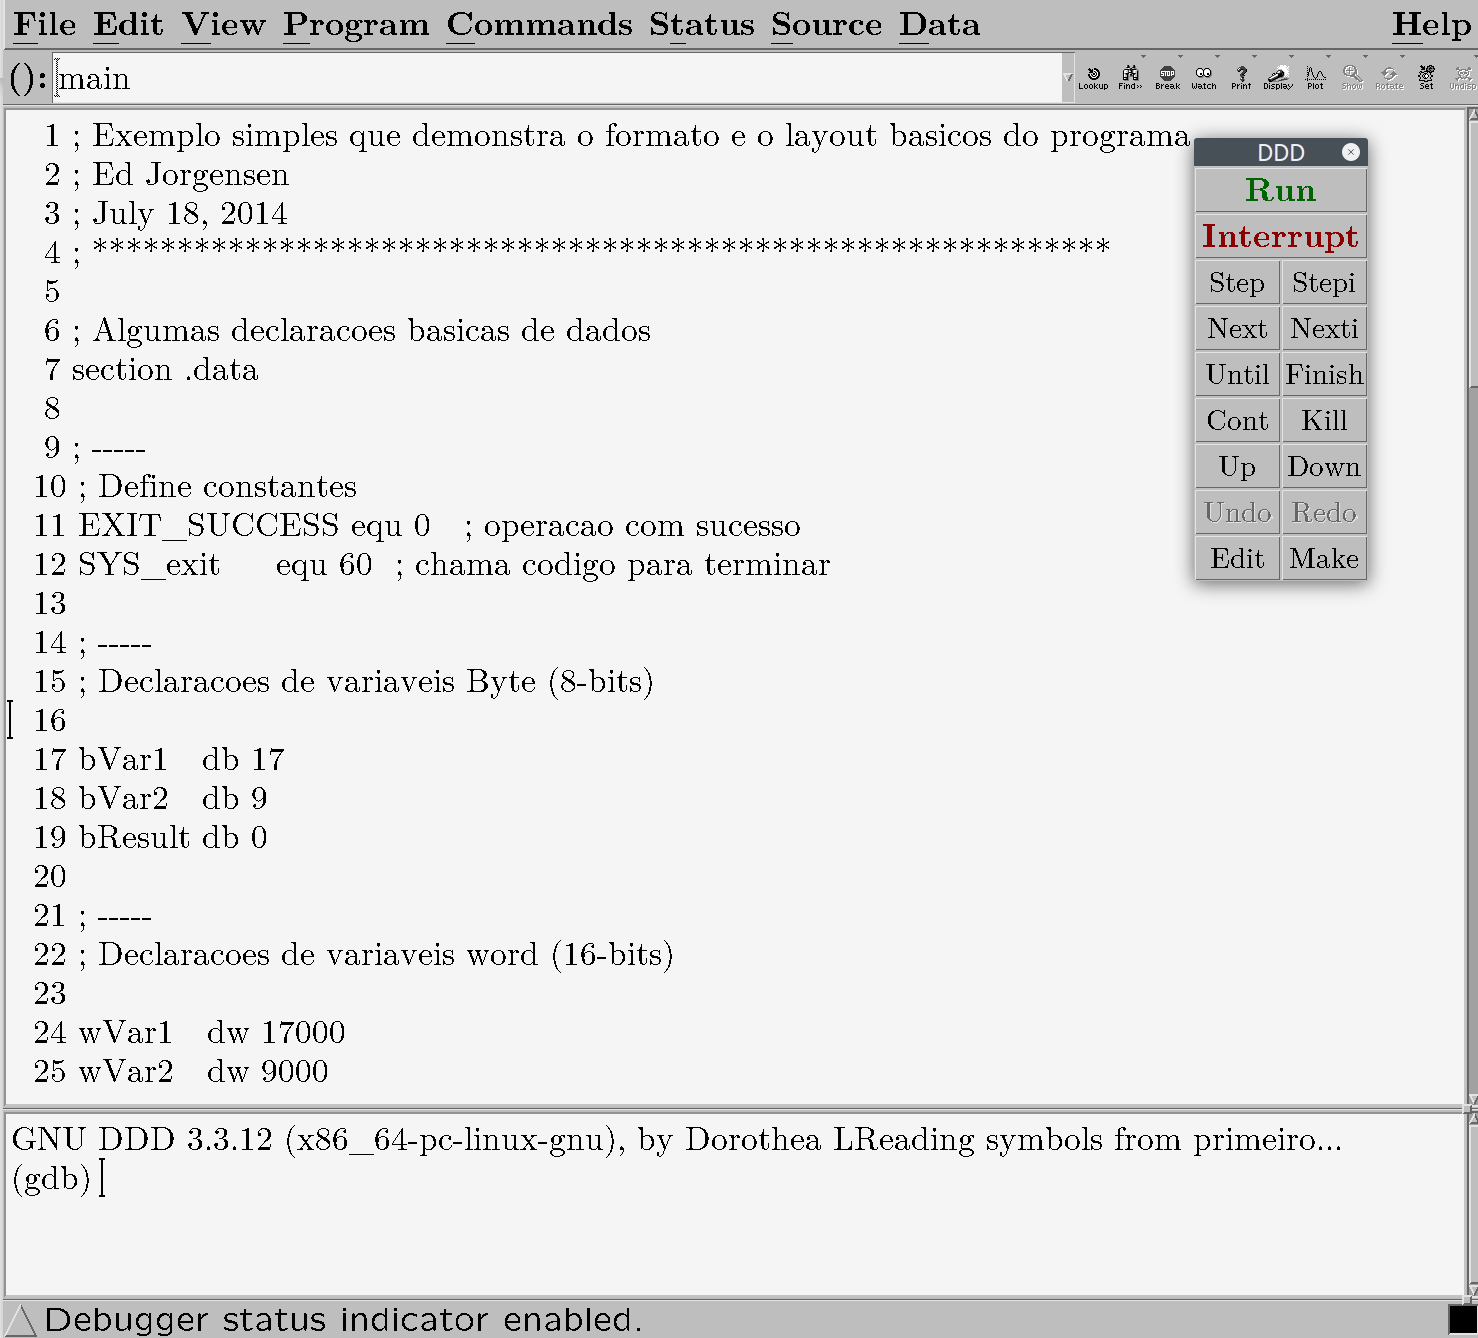
\includegraphics[width=0.8\linewidth]{imagens/ddd01}
\end{center}
	\caption{Tela inicial do depurador.}
\end{figure}

Se o código não for exibido de maneira semelhante à mostrada acima, as etapas de montagem e vinculação devem ser verificadas. Especificamente, o qualificador \textbf{-g} deve ser incluído nas etapas de montagem e de link.

A ajuda integrada está disponível clicando no item de menu \textbf{Help} (canto superior direito). Os manuais \textbf{DDD} e \textbf{GDB} estão disponíveis nas páginas dos respectivos desenvolvedores. Para sair do DDD/GDB, selecione \textbf{File} $\rightarrow$ \textbf{Exit} (na barra de menu superior).

\subsection{Definições de configuração DDD}
Algumas sugestões adicionais de configurações de \textbf{DDD/GDB} incluem:

\begin{itemize}
	\item \textbf{Edit $\rightarrow$ Preferences $\rightarrow$ General $\rightarrow$ Suppress X Warning}
	\item \textbf{Edit $\rightarrow$ Preferences $\rightarrow$ Source $\rightarrow$ Display Source Line Numbers}
\end{itemize}

Eles não são obrigatórios, mas podem facilitar o uso do depurador. Se definido, as opções serão salvas e lembradas para usos sucessivos do depurador (na mesma máquina).

\section{Execução de programa com DDD}
Para executar o programa, clique no botão \textbf{Run} no menu da ferramenta de comando (mostrado abaixo). Como alternativa, você pode digitar \textbf{run} no prompt \textbf{(gdb)} (janela inferior do console \textbf{GDB}). No entanto, isso executará o programa inteiramente e, quando feito, os resultados serão zerados (e perdidos).

\subsection{Definindo pontos de interrupção}
Para controlar a execução do programa, será necessário definir um \textit{breakpoint} (local de pausa de execução) para pausar o programa em um local selecionado pelo usuário. Isso pode ser feito selecionando o local de origem (linha para parar). Para este exemplo, vamos parar na linha 31.

O ponto de interrupção pode ser feito de três maneiras:\begin{itemize}
	\item Clique com o botão direito no número da linha e selecione: \textit{Set Breakpoint}
	\item No console de comando GDB, no prompt (gdb), digite: \textbf{break last}
	\item No console de comando GDB, no prompt (gdb), digite: \textbf{break 88}
\end{itemize}

No exemplo a seguir, a linha 87 é um rótulo sem instrução. Se um ponto de interrupção for definido no rótulo, ele irá parar na próxima instrução executável (linha 88 neste exemplo).

Quando configurado corretamente, o ícone ``stop'' aparecerá ao lado do número da linha (conforme mostrado no diagrama).

\begin{figure}[h]
	\begin{center}
		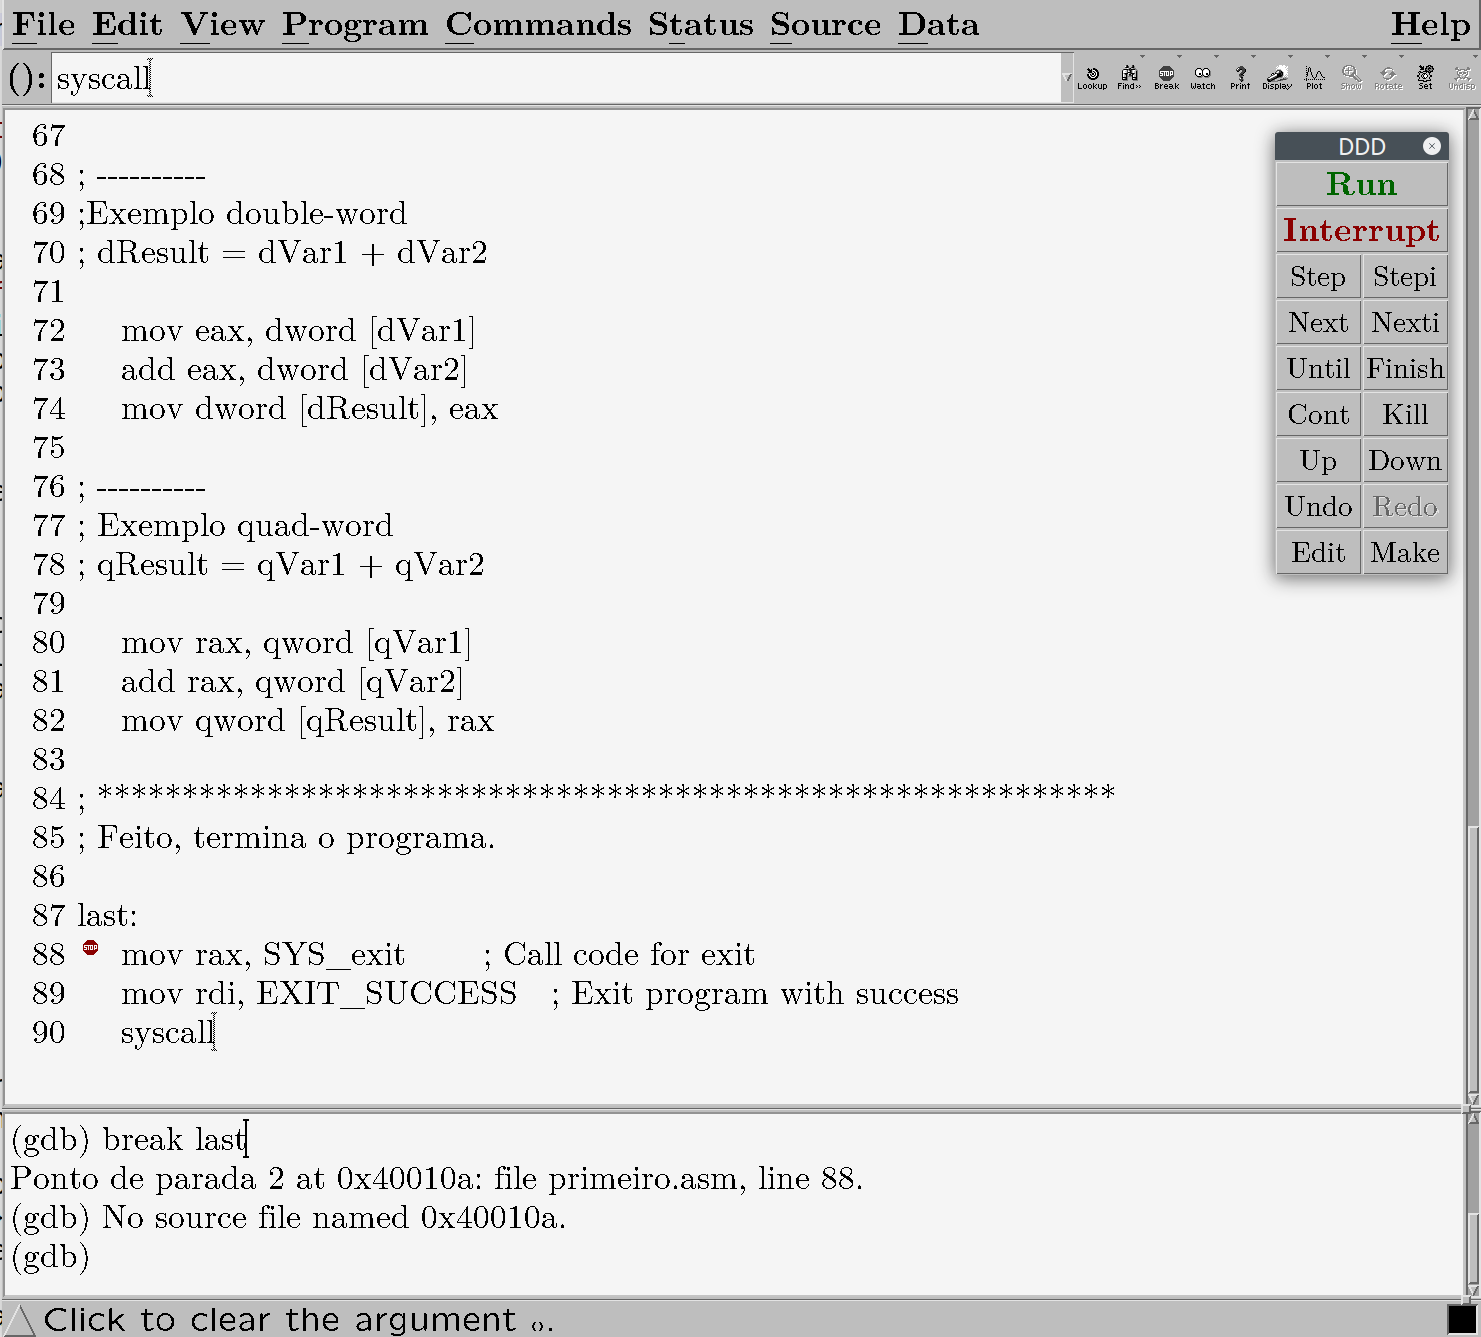
\includegraphics[width=0.8\linewidth]{imagens/dddbreakpoint}
	\end{center}
	\caption{Tela do debugger com breakpoint.}
\end{figure}

Os comandos \textbf{DDD/GDB} podem ser digitados na janela inferior (no \textit{prompt (gdb)}) a qualquer momento. Vários pontos de interrupção podem ser definidos, se desejado.

\subsection{Executando Programas}
Uma vez que o depurador é iniciado, a fim de usar efetivamente o depurador, um ponto de interrupção inicial deve ser definido.

Depois que o ponto de interrupção é definido, o comando de execução pode ser executado clicando na janela do menu \textbf{Run} ou digitando \textbf{run} no prompt (gdb). O programa será executado até, \textit{mas não incluindo}, a instrução com a seta verde.

\begin{figure}[h]
	\begin{center}
		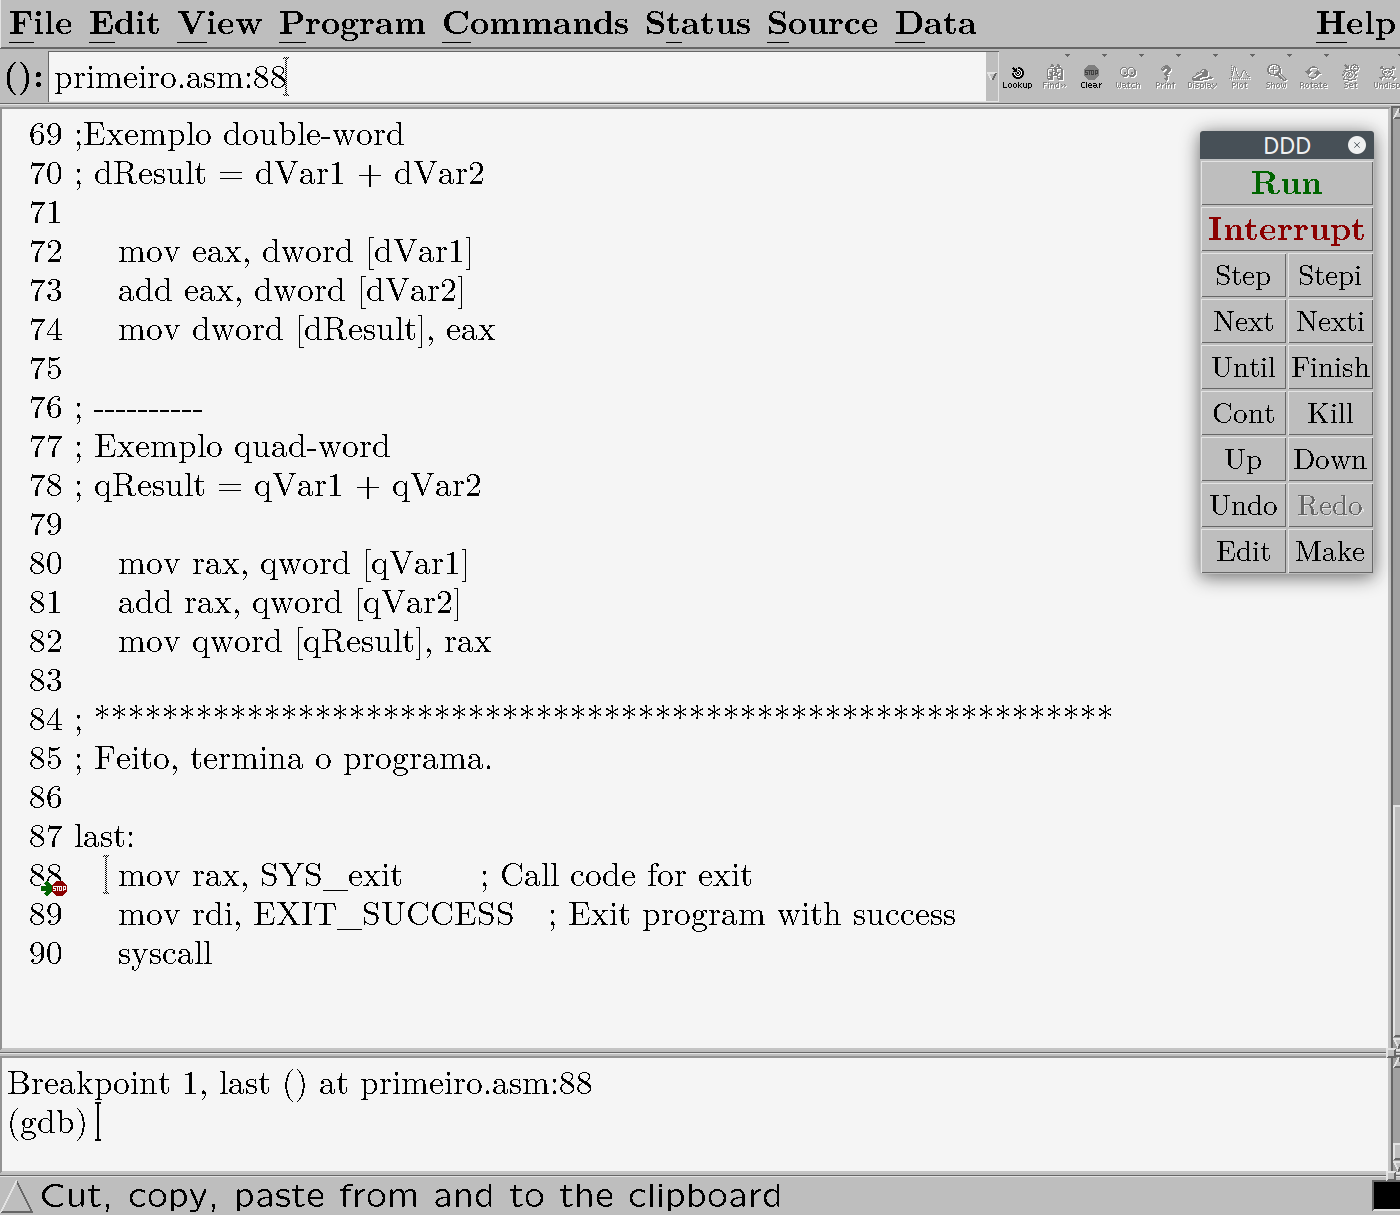
\includegraphics[width=0.8\linewidth]{imagens/ddd03}
	\end{center}
	\caption{Tela do debugger com seta verde.}
\end{figure}

O ponto de interrupção é indicado com o sinal de parada à direita (consulte o exemplo anterior). A localização atual é indicada com uma seta verde. Especificamente, a seta verde aponta para a próxima instrução a ser executada. Ou seja, a instrução apontada pela seta verde ainda não foi executada.

\subsubsection{Run/Continue}
Conforme necessário, pontos de interrupção adicionais podem ser definidos. No entanto, clique no comando \textbf{Run} para reiniciar a execução do início e parar no ponto de interrupção inicial.

\begin{figure}[h]
	\begin{center}
		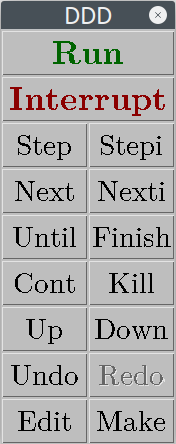
\includegraphics[width=0.12\linewidth]{imagens/ddd04}
	\end{center}
	\caption{Barra de comandos do DDD.}
\end{figure}

Após o comando \textbf{Run} inicial, para continuar para o próximo ponto de interrupção, o comando continue deve ser usado (clicando na janela do menu \textbf{Cont} ou digitando \textbf{cont} no prompt (gdb)). Linhas únicas também podem ser executadas uma linha por vez digitando os comandos passo ou próximo  (clicando em \textbf{Step} ou \textbf{Next} na janela de menu ou digitando \textbf{step} ou \textbf{next} no prompt (gdb)).


\subsubsection{Next/Step}
O comando \textbf{next} executa a próxima instrução. Isso inclui a execução de uma função inteira, se necessário. O comando \textbf{step} executará uma etapa, entrando nas funções se necessário. Para uma única instrução sem função, não há diferença entre os comandos \textbf{next} e \textbf{step}.

\subsection{Exibindo Conteúdo de Registradores}
O método mais simples de ver o conteúdo dos registradores é usar a janela de registradores. A janela de registradores não é exibida por padrão, mas pode ser visualizada selecionando \textbf{Status} $\rightarrow$ \textbf{Registers} (na barra de menu superior). Quando exibida, a janela de registro mostrará o conteúdo do registradores por nome do registrador (coluna da esquerda), em hexadecimal (coluna do meio) e decimal com sinal (coluna da direita).

\begin{figure}[h]
	\begin{center}
		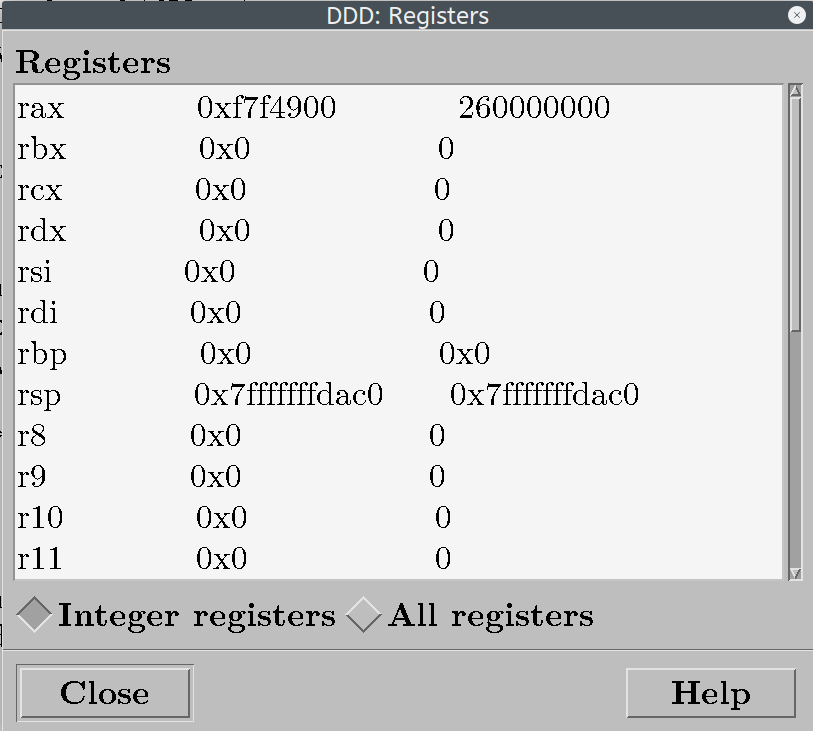
\includegraphics[width=0.5\linewidth]{imagens/ddd05}
	\end{center}
	\caption{Janela de registradores.}
\end{figure}

Dependendo da máquina e da resolução da tela, a janela de registradores pode precisar ser redimensionada para visualizar todo o conteúdo.

A terceira coluna da janela de registradores geralmente mostra a representação decimal de palavras quádruplas, exceto para alguns registradores de propósito especial (\textbf{rbp} e \textbf{rsp}). A representação decimal com quatro palavras com sinais nem sempre é significativa. Por exemplo, se dados não assinados estiverem sendo usados (como endereços), a representação com sinal estará incorreta. Além disso, quando dados de caractere são usados, a representação com sinal não seria significativa.

Por padrão, apenas os registradores inteiros são exibidos. Clicar na caixa ``All registers'' adicionará os registros de ponto flutuante ao \textit{display}. A visualização exigirá rolar para baixo na janela de registradores.

\subsection{Resumo de comandos DDD/GDB}
A tabela a seguir fornece um pequeno subconjunto dos comandos \textbf{DDD} mais comuns. Quando digitados, a maioria dos comandos pode ser abreviada. Por exemplo, \textbf{quit} pode ser abreviado como \textbf{q}. O comando e a abreviatura são mostrados na Tabela \ref{tab:comandosddd}.

\begin{table}[ht]
	\begin{center}
	\resizebox{0.6\textwidth}{!}{%
	\begin{tabular}{|ll|}
	\hline
	\rowcolor[HTML]{C0C0C0}
	\textbf{Comando} & \textbf{Descrição} \\ \hline
	\textbf{quit |q} & Sai do depurador. \\ \hline
	\textbf{break <label/addr>}  & Define um \textit{breakpoint} (ponto de parada) \\ 
	\textbf{| b <label/addr>} & em \textbf{<label>} ou	\textbf{<address>}. \\\hline	
	\textbf{run <args> | r <args>} & Execute o programa (até o primeiro \\
	& ponto de parada).\\ \hline
	\textbf{continue | c} & Continue a execução (até o próximo\\
	&  ponto de parada).\\ \hline
	\textbf{continue <n> | c <n>} & Continue a execução (até o próximo\\
	& ponto de parada), ignorando\\
	& n-1 passagens do ponto de parada.\\
	& Isso pode ser usado para chegar rapida-\\
	&mente à n-ésima iteração de um loop.\\ \hline
	\textbf{step | s} & Passe para a próxima instrução\\
	& (ou seja, siga as chamadas\\
	& de função/procedimento)\\ \hline
	\textbf{next | n }& Próxima instrução (não entra em\\
	& funções/chamadas de procedimento).\\ \hline
	\textbf{F3} & Reinicie o programa (e pare no\\
	& primeiro ponto de parada).\\\hline
	\textbf{where} & Ativação atual (profundidade\\
	& da chamada).\\ \hline
	\textbf{x/<n><f><u> \$rsp} & Examine o conteúdo da pilha.\\ \hline
	\textbf{x\/<n><f><u> \&<var>} & Examine a localização da memória\\
	& <var>. <n> número de locais\\
	& a serem exibidos, 1 é o padrão.\\
	&\begin{tabular}{ll}
		\textbf{<f> formato}: &d - decimal (com sinal)\\
	    &x - hex\\
	    &u - decimal (sem sinal)\\
	    &c - caractere\\
	    &s - string\\
	    &f - ponto flutuante\\	
	\end{tabular}\\
	& \textbf{<u> tamanho da unidade}: \\
	&\begin{tabular}{ll}
		&b - byte (8 bits)\\
	\hspace{2.55cm}	& h - halfword (16-bits)\\
		& w - word (32-bits)\\
        & g - gigante (64-bits) \\
	\end{tabular}\\	\hline
	source <filename> & Leia os comandos do arquivo \textbf{<filename>}.\\\hline
	\textbf{set logging file <filename>}& Defina o arquivo de registro como\\
	& \textbf{<filename>}, o padrão é gdb.txt.\\\hline
	\textbf{set logging on} & Ative o registro (para um arquivo). \\\hline
	\textbf{set logging off}	& Desative o registro (para um arquivo). \\\hline
	\textbf{set logging overwrite}&Quando o registro (para um\\
	& arquivo) estiver ativado, substitua o\\
	&arquivo de registro anterior (se houver). \\\hline
\end{tabular}}
\end{center}
	\caption{Comandos DDD.}
	\label{tab:comandosddd}
\end{table}

Mais informações podem ser obtidas por meio do recurso de ajuda integrado ou da documentação no site do \textbf{ddd} (referenciado no Capítulo \ref{cap1}.

\subsubsection{Comandos DDD/GDB, exemplos}
Por exemplo, dadas as declarações de dados abaixo:

\lstinputlisting{source/exemplo1.asm}

Assumindo dados com sinal, os comandos para examinar as instruções de memória seriam os seguintes:
\begin{verbatim}
x/db &bnum1
x/dh &wnum2
x/dw &dnum3
x/dg &qnum
x/s &class
x/f &twopi
\end{verbatim}

Se um comando de exame de memória (\textit{memory dump}) inadequado for usado (ou seja, tamanho incorreto), não haverá mensagem de erro e o depurador exibirá o que foi solicitado (mesmo que não faça sentido). O exame das variáveis exigirá o uso do comando de exame de memória  apropriado com base nas declarações de dados. As opções adicionais podem ser acessadas no menu na parte superior da tela.

Para exibir um \textit{array} em \textbf{DDD}, o comando básico de exame de memória é usado.
\begin{center}
	\textbf{x/<n><f><u> \&<variable>}
\end{center}

Por exemplo, assumindo a declaração de:
\begin{lstlisting}
list1	dd	100001, -100002, 100003, 100004, 100005
\end{lstlisting}

O comando de exame de memória seria o seguinte:\\
\textbf{x/5dw \&list1}

Onde o \textbf{5} é o comprimento do array. O \textbf{d} indica dados com sinal (\textbf{u} teria sido dados sem sinal). O \textbf{w} indica dados de tamanho de \textbf{32 bits} (que é o que a definição \textbf{dd}, \textit{define double}, declara no arquivo de origem). O \textbf{\&list1} se refere ao endereço da variável. Observe que o endereço aponta para o primeiro elemento (e apenas o primeiro elemento). Como tal, é possível exibir menos ou mais elementos que são realmente declarados no array.

O comando básico para examinar a memória pode ser usado diretamente com um endereço de memória (em oposição a um nome de variável). Por exemplo:\\
\textbf{x/dw 0x600d44}

Os endereços são normalmente exibidos em hexadecimal, portanto, um \textbf{0x} seria necessário para inserir o endereço hexadecimal diretamente, conforme mostrado.

\subsection{Exibindo o conteúdo da pilha}
Existem algumas ocasiões em que a exibição do conteúdo da pilha pode ser útil. A pilha é normalmente composta de elementos não sinalizados de 64 bits. O comando para exame de memória é usado, porém o endereço está no registrador \textbf{rsp} (não é um nome de variável). O comando de exame de memória para exibir o topo atual da pilha seria o seguinte:\\
\textbf{x/ug \$rsp}

O comando de exame de memória para exibir os 6 itens do topo na pilha seria o seguinte:\\
\textbf{x/6ug \$rsp}

Devido à implementação da pilha, o primeiro item mostrado sempre será o topo atual da pilha.

\subsection{Arquivo de comandos do depurador}
Como os comandos de exibição de dados devem estar corretos (já que não há erro), pode ser entediante. Para ajudar a reduzir os erros, a execução correta e o comando de exibição podem ser armazenados em um arquivo de texto. O depurador pode então ler os comandos do arquivo (em vez de digitá-los manualmente). Embora os resultados sejam normalmente exibidos na tela, os resultados podem ser redirecionados para um arquivo de saída. Isso pode ser útil para uma revisão fácil.

Por exemplo, alguns comandos típicos do depurador para definir o ponto de interrupção, executar o programa, exibir algumas variáveis e redirecionar a saída para um arquivo de log podem ser os seguintes:

\lstinputlisting{source/script1.txt}
\textit{Nota 1}; este exemplo assume que um rótulo '\textbf{last}' é definido no programa de origem (como é feito no programa de exemplo).

\textit{Nota 2}; este exemplo sai do depurador. Se isso não for desejado, o comando 'quit' pode ser removido. Ao sair do arquivo de entrada, o depurador pode solicitar a confirmação do usuário da saída (sim ou não).

Esses comandos devem ser colocados em um arquivo (como \textit{gdbIn.tx}t), para que possam ser lidos a partir do depurador.

\subsubsection{Arquivo de comandos do depurador (interativo)}
O comando do depurador para ler um arquivo é ''source <filename>''. Por exemplo, se o nome do arquivo de comando for gdbIn.txt,\\
	\textbf{(gdb) source gdbIn.txt}

Com base nos comandos acima, a saída será colocada no arquivo \textit{out.txt}. O nome do arquivo de saída pode ser alterado conforme desejado.

Cada programa exigirá um conjunto de comandos de entrada personalizado com base nas variáveis e tamanhos associados. O arquivo de comandos de entrada do depurador só será útil quando o programa estiver quase funcionando. Travamentos do programa e outros erros mais significativos exigirão depuração interativa para determinar o erro específico.

\subsubsection{Arquivo de comandos do depurador (não interativo)}
É possível obter o arquivo de saída diretamente sem uma sessão \textbf{DDD} interativa. O comando a seguir, inserido na linha de comando, executará o comando no arquivo de entrada do programa fornecido, criará o arquivo de saída e sairá do programa.\\
\textbf{gbd <gdbIn.txt prog}\\
Que criará o arquivo de saída (conforme especificado no arquivo \textit{gdbIn.txt}) e sairá do depurador. Esta é a opção mais rápida para obter o arquivo de saída final para um programa em funcionamento. Novamente, isso só seria útil se o programa estiver funcionando ou muito perto de funcionar corretamente.

\section{Exercícios}
Abaixo estão algumas perguntas baseadas neste capítulo.

\subsection{Questionário}
\begin{enumerate}
	\item Como o depurador é iniciado (na linha de comando)?
	\item Qual opção é necessária durante a etapa de montagem e vinculação para garantir o	programa ser facilmente depurado.
	\item O que o comando \textbf{run} faz especificamente?
	\item O que o comando \textbf{continue} faz especificamente?
	\item Como a janela de registradores é exibida?
	\item Existem três colunas na janela de registradores. O primeiro mostra o registrador.	O que as outras duas colunas mostram?
	\item Uma vez que o depurador é iniciado, como o usuário pode sair?
	\item Descreva como um ponto de parada é definido (várias maneiras).
	\item Qual é o comando debugger para ler os comandos debugger de um arquivo?
	\item Quando o DDD mostra uma seta verde apontando para uma instrução, o que isso significa?
	\item Forneça o comando debugger para exibir cada uma das seguintes variáveis em decimal.
	\begin{enumerate}
		\item \textbf{bVar1} (variável de tamanho de byte)
		\item \textbf{wVar1} (variável de tamanho de palavra)
		\item \textbf{dVar1} (variável de tamanho de palavra dupla)
		\item \textbf{qVar1} (variável de tamanho de palavra quádrupla)
		\item \textbf{bArr1} (matriz de 30 elementos de bytes)
		\item \textbf{wArr1} (matriz de palavras com 50 elementos)
		\item \textbf{dArr1} (matriz de 75 elementos de palavras duplas)
	\end{enumerate}
    \item Forneça o comando debugger para exibir cada uma das seguintes variáveis em formato hexadecimal.
    \begin{enumerate}
    	\item \textbf{bVar1} (variável de tamanho de byte)
    	\item \textbf{wVar1} (variável de tamanho de palavra)
    	\item \textbf{dVar1} (variável de tamanho de palavra dupla)
    	\item \textbf{qVar1} (variável de tamanho de palavra quádrupla)
    	\item \textbf{bArr1} (matriz de 30 elementos de bytes)
    	\item \textbf{wArr1} (matriz de palavras com 50 elementos)
    	\item \textbf{dArr1} (matriz de 75 elementos de palavras duplas)
    \end{enumerate}
    \item  Qual é o comando do depurador para exibir o valor no topo da pilha atual?
    \item Qual é o comando debugger para exibir cinco (5) valores no topo da pilha atual?
\end{enumerate}

\subsection{Projetos sugeridos}
Abaixo estão alguns projetos sugeridos com base neste capítulo.
\begin{enumerate}
	\item Digite o programa de exemplo do Capítulo \ref{cap4:formato}, Formato do programa. Monte e conecte o programa conforme descrito no Capítulo \ref{Ferramentasdedesenvolvimento}, Ferramentas de desenvolvimento. Execute o depurador conforme observado neste capítulo. Defina um ponto de interrupção no último rótulo e execute o programa (para esse ponto de interrupção). Verifique interativamente se os cálculos realizados resultaram nos valores corretos. Isso exigirá a digitação dos comandos de memória de exame do depurador apropriados (com base no tamanho da variável).
	\item Depois de concluir o problema anterior, crie um arquivo de entrada do depurador que definirá o envio da saída para um arquivo de texto, definirá um ponto de interrupção, executará o programa e exibirá os resultados para cada variável (com base no tamanho de variável apropriado). Execute o depurador e leia o arquivo de origem. Verifique se o arquivo de entrada funcionou corretamente e se os cálculos do programa estão corretos com base nos resultados mostrados no arquivo de saída.
	\item Crie um arquivo de script de montagem e link, conforme descrito no Capítulo \ref{Ferramentasdedesenvolvimento}, Ferramentas de desenvolvimento. Use o script para montar e linkar o programa. Certifique-se de que o script monte e link corretamente.
\end{enumerate}

